\documentclass[main.tex]{subfiles}
\begin{document}
在物理问题中经常碰到的情况是,物理量$f$随空间位置和时间变化,故$f$是空间位置向量$\mathbf{r}$和时间$t$的函数$f\left(\mathbf{r},t\right)$。在直角坐标系$\left(x,y,z\right)$下可写作$f\left(x,y,z,t\right)$。在一维问题中写作$f\left(x,t\right)$。因此,主导这一物理量$f$的变化规律的方程,既需要规定f随时间变化的规律——$f$的时间偏导数$\partial f/\partial t$、$\partial^2 f/\partial t^2$、……,又要规定$f$随空间位置变化的规律——$f$的梯度和更高阶的空间导数$\boldsymbol{\nabla}f=\left(\partial f/\partial x, \partial f/\partial y,\partial f/\partial z\right)$、……,因此将含有$f$的偏导数。

\emph{偏微分方程(partial differential equation,PDE)}是这样的一类方程:
\begin{itemize}
    \item 它含有两个或两个以上独立自变量(例如$x,y,z,t$);
    \item 一个依赖这些变量的未知函数(例如$f=f\left(x,y,t,z\right)$);
    \item 以及该函数对这些变量的偏导函数(例如$\partial f/\partial t$、$\partial f/\partial x$、$\partial^2 f/\partial x^2$……)。
\end{itemize}

微分方程的基本术语\cite[\S 10]{华工高数2009下},可以自动适用于偏微分方程。例如,方程所含有的偏微分的最高阶数,称作该\emph{偏微分方程的阶}。如果某个函数及其各阶偏导函数代入偏微分方程能使后者成为恒等式,则称这个函数为\emph{偏微分方程的一个解}。如果一个偏微分方程\emph{所有}解可以用一个通式表示出来,这个通式就叫做这个\emph{偏微分方程的通解}。

一个关于某物理过程的偏微分方程,只有给定了\emph{初始条件(initial condition,IC)}和\emph{边界条件(boundary conditions,BCs)},才能得到具体的、不偏待定参数的解,以对应于一个具体的物理问题的预测。初始条件是指未知函数$f\left(x,y,z,t\right)$限制在时间$t=0$时的函数$f\left(x,y,z,0\right)\equiv f_0\left(x,y,z\right)$及其偏导函数的性质。边界条件是在未知函数$f\left(\mathbf{r},t\right)$限制在这一物理问题所关心的空间区域$\Omega$的边界$\partial\Omega$(也需指明)上的函数$f\left(\mathbf{r},t\right),\mathbf{r}\in\partial\Omega$及其偏导函数的性质\footnote{在偏微分方程的数学理论中,由于不区分自变量是时间还是空间位置等物理意义,故一律都称作边界条件。}。在具体的初始条件和边界条件规定下,仍满足偏微分方程的解,称为该\emph{偏微分方程在给定初始条件和边界条件下的特解}。

\begin{example}[传热方程]
    关于温度$u\left(\mathbf{r},t\right)$的方程
    \[
        \frac{\partial u}{\partial t}=k\nabla^2u,\quad k=\text{常数}
    \]
    称为传热方程(heat equation)。其中$\nabla^2 u\left(x,y,z,t\right)\equiv\partial^2 u/\partial x^2+\partial^2 u/\partial y^2+\partial^2 u/\partial z^2$。规定了如下例所示的初始条件和边界条件之后,可理解为如图\ref{fig:heat_eq_sol}所示的物理问题。
    \begin{align*}
        \text{方程:}   & \frac{\partial u}{\partial t}=k\frac{\partial^2 u}{\partial x^2},\quad 0\leq x\leq 1,\quad t\geq 0 \\
        \text{边界条件:} & u\left(0,t\right)=u\left(1,t\right)=0,\quad\forall t\geq 0                                         \\
        \text{初始条件:} & u\left(x,0\right)=u_0\left(x\right),\quad 0\leq x\leq 1
    \end{align*}
    其中$u_0\left(x\right)$是某个给定表达式的函数。例如,当$u_0\left(x\right)=\sin\left(\pi x\right)$时,上述边界条件和初始条件规定下方程的特解是$u\left(x,t\right)=e^{-\pi^2kt}\sin\left(\pi x\right)$。它在$k=0.01$时的图像如图\ref{fig:heat_eq_sol}所示。
\end{example}

\begin{figure}[ht]
    \centering
    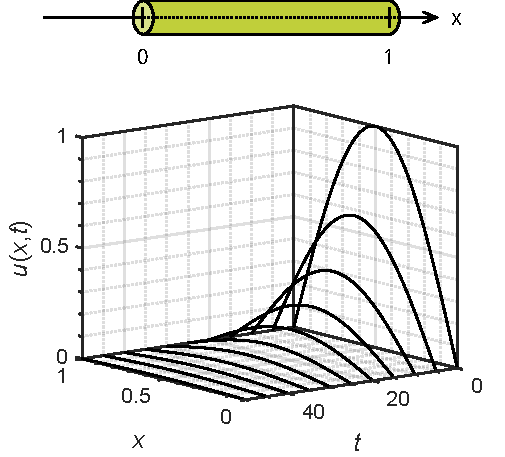
\includegraphics{../images/heat_eq_sol.pdf}
    \caption{一根长为1、左端置于原点处的一维直棒,在$t=0$时、温度在棒上的分布是$u_0\left(x\right)=\sin\left(\pi x\right)$。若棒的两端温度恒定为0,即$u\left(0,t\right)=u\left(1,t\right)=0\forall t\geq 0$,传热系数$k=0.01$,那么棒上的温度分布如何随时间演变?}
    \label{fig:heat_eq_sol}
\end{figure}

% ==========================================
\section{一阶偏微分方程}
一阶偏微分方程的一般形式是:
\[
    F\left(x_1,x_2,\cdots,x_n;f;\frac{\partial}{\partial x_1}f,\cdots,\frac{\partial}{\partial x_n}f\right)=0,\quad n>1
\]
在具体问题中,函数$F$的形式是给定的,函数$f$是未知函数。为简化考虑,以下以维数$n=2$为例继续讨论,即未知函数$f=f\left(x,y\right)$。如果一个一阶偏微分方程可以具体写成形如
\begin{equation}\label{eq:linear_PDE}
    P\left(x,y,f\right)\frac{\partial f}{\partial x}+Q\left(x,y,f\right)\frac{\partial f}{\partial y}=R\left(x,y,f\right)
\end{equation}
的形式,则为一阶拟线性(quasilinear)偏微分方程;当函数$P$、$Q$不依赖未知函数$f$时,则为一阶半线性(semilinear)偏微分方程;当函数$P$、$Q$、$R$都不依赖特征函数$f$时,则为一阶线性(linear)偏微分方程。如果上式符合一阶线性偏微分方程要求且$R=0$,则称方程是齐次的(homogeneous),否则称其为非齐次的(nonhomogeneous)。以下我们专门讨论一阶线性偏微分方程。

常微分方程组
\[
    \frac{dx}{P\left(x,y,f\right)}=\frac{dy}{Q\left(x,y,f\right)}=\frac{df}{R\left(x,y,f\right)}
\]
称方程\eqref{eq:linear_PDE}的特征方程组。解第1个等号得$x/P=y/Q+C_1$,解第二个等号得$y/Q=f/R+C_2$。可验证,给定任意函数$\Psi\left(u\right)$,$C_2=\Psi\left(C_1\right)$是方程\eqref{eq:linear_PDE}的通解,即
\[
    \frac{y}{Q}-\frac{f}{R}=\Psi\left(\frac{x}{P}-\frac{y}{Q}\right)\Leftrightarrow f=\frac{Ry}{Q}-R\Psi\left(\frac{x}{P}-\frac{y}{Q}\right)
\]
是方程\eqref{eq:linear_PDE}的通解。
\end{document}